\documentclass{article}
\usepackage{setspace,tikz,wrapfig}
\usepackage[text={6.5in,8.5in},centering]{geometry}
\geometry{verbose,a4paper,tmargin=2.4cm,bmargin=2.4cm,lmargin=2.4cm,rmargin=2.4cm}
\usepackage{graphicx,amsmath,cases,multirow,appendix,graphicx,xcolor}

\setlength\parindent{0pt}

\newcommand{\note}[1]{\colorbox{gray!30}{#1}}
\newcommand{\ind}{\-\hspace{1cm}}
\newcommand*\circled[1]{\tikz[baseline=(char.base)]{
            \node[shape=circle,draw,inner sep=2pt] (char) {#1};}}
\newenvironment{rcases}
  {\left.\begin{aligned}}
  {\end{aligned}\right\rbrace} 
  
  
\renewcommand\floatpagefraction{.9}
\renewcommand\topfraction{.9}
\renewcommand\bottomfraction{.9}           


\begin{document}

\noindent\makebox[\textwidth][c]{\Large\bfseries Lecture 13 -- Eigenvalues}

\textbf{Concepts:}\\
\ind - Eigenvalues\\
\ind - Matrix determinant
\ind - Complex numbers\\

\rule[0.5ex]{\linewidth}{1pt}

\textbf{Matrix Algebra \& Conventions}
\begin{center}
\textbf{A} - matrix (bold) \ind \ind $\vec w$ - vector (italicized) \ind \ind $A_{ij}$ or $w_i$ - scalars\\
$\begin{bmatrix} a\\ b \end{bmatrix}$ - column vector \ind \ind $\begin{bmatrix} a & b \end{bmatrix}$ - row vector
\end{center}

\rule[0.5ex]{\linewidth}{1pt}

\textbf{Why do eigenvalues indicate stability properties?}
\begin{center}
\begin{tabular}{ll}
\hline
\textbf{Eigenvalues ($\lambda_i$)} & \textbf{Interpretation} \\ 
\hline
 $Re(\lambda_i)< 0$  for all $i$& Stable node\\ 
  $Re(\lambda_i)< 0$ for some $i$ & Saddle node \\ 
 $Re(\lambda_i)> 0$ for all $i$ & Unstable node \\ 
 $Re(\lambda_i) = 0$ for all $i$ & Neutrally stable \\ 
 \hline
  $Im(\lambda_i) = 0$ for all $i$ & No oscillations \\ 
 $Im(\lambda_i) \neq 0$ for some $i$  & Oscillations \\ 
 \hline
\end{tabular} 
\end{center}
\begin{center}
	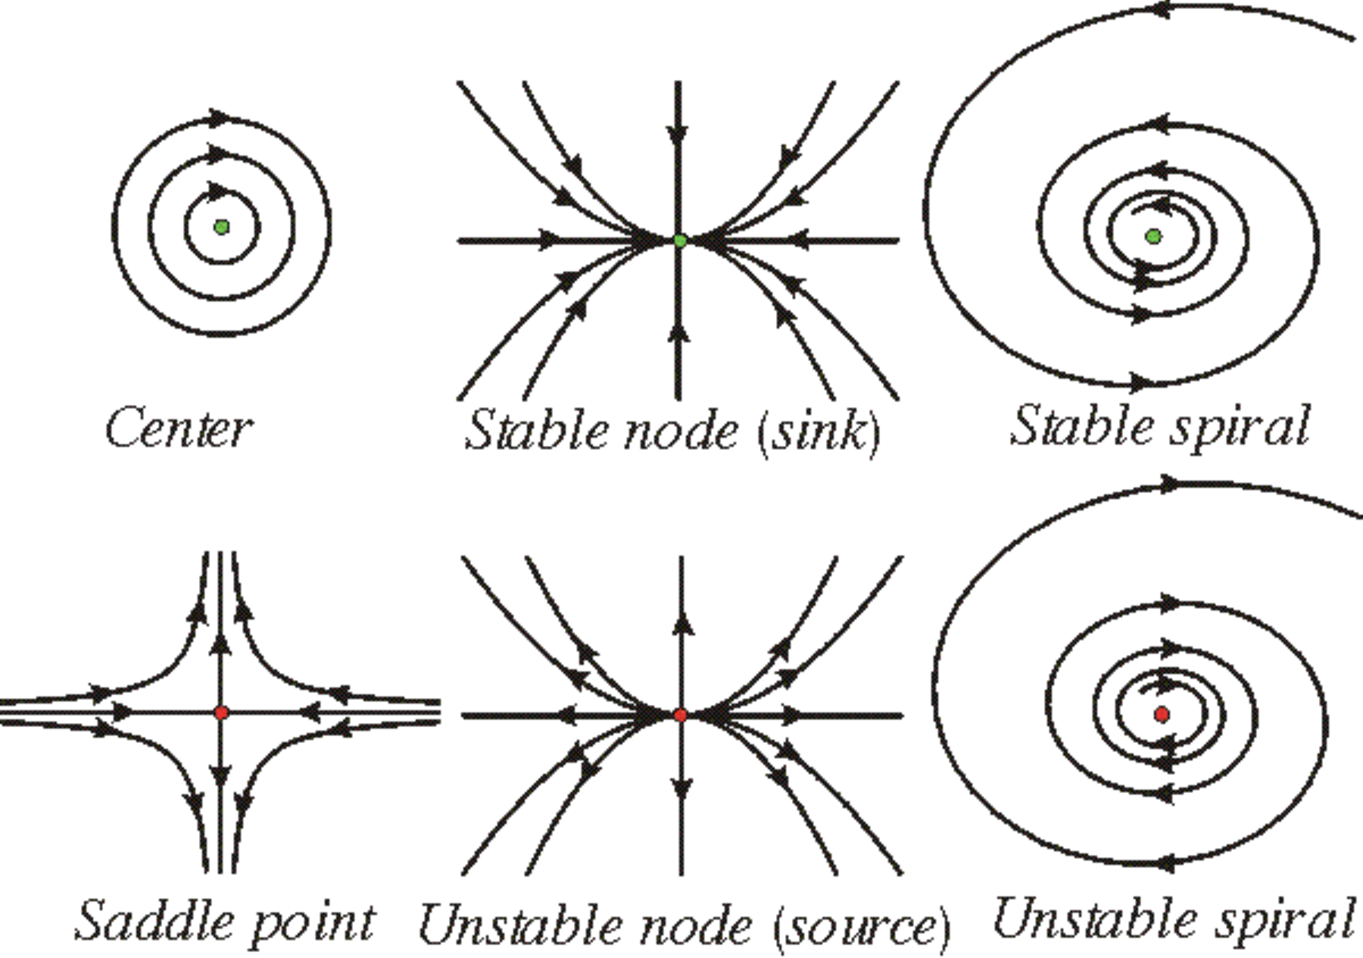
\includegraphics[width=7cm]{figs/Points.pdf}
	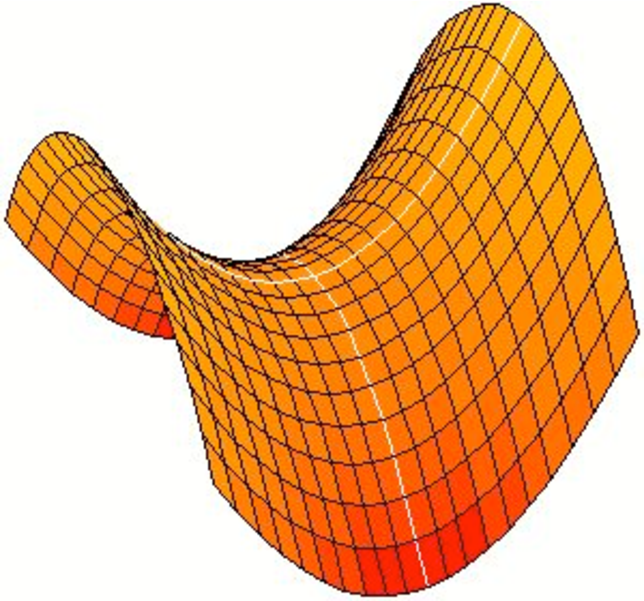
\includegraphics[width=3cm]{figs/Saddle.pdf}
\end{center}
Recall, for perturbations $x$ and $y$ to species $u_1$ and $u_2$:
\begin{equation*}
	\frac{d x}{dt}=f_1(u_1^* + x, u_2^* + y)\approx \underbrace{\left. \frac{\partial f_1}{\partial u_1}\right|_{u_1^*, u_2^*}}_{A_{11}} \cdot x + \underbrace{\left. \frac{\partial f_1}{\partial u_2}\right|_{u_1^*, u_2^*}}_{A_{12}} \cdot y
\end{equation*}
and
\begin{equation*}
	\frac{d y}{dt}=	f_2(u_1^* + x, u_2^* + y)\approx \underbrace{\left. \frac{\partial f_2}{\partial u_1}\right|_{u_1^*, u_2^*}}_{A_{21}} \cdot x + \underbrace{\left. \frac{\partial f_2}{\partial u_2}\right|_{u_1^*, u_2^*}}_{A_{22}} \cdot y
\end{equation*}

Therefore, if $x$ and $y$ are small, can approximate dynamics as
\begin{align*}
	\frac{dx}{dt}&=A_{11} \cdot x + A_{12} \cdot y\\	
	\frac{dy}{dt}&=A_{21} \cdot x + A_{22} \cdot y
\end{align*}

In matrix form:
\begin{equation*}
	\underbrace{\begin{bmatrix}\frac{dx}{dt} \\ \frac{dy}{dt}\end{bmatrix}}_{\frac{d \vec{n}}{dt}} = \underbrace{ \begin{bmatrix}A_{11} & A_{12}\\ A_{21} & A_{22}\end{bmatrix}}_{\mathbf{A}} \cdot \underbrace{\begin{bmatrix}x \\ y\end{bmatrix}}_{\vec{n}}
\end{equation*}
or equivalently
\begin{equation*}
	\frac{d \vec{n}}{dt}= \mathbf{A} \cdot \vec{n}
\end{equation*}

\rule[0.5ex]{\linewidth}{1pt}
\textbf{Side note:}\\
Matrix addition:
\begin{equation*}
 \begin{bmatrix} a & b \\ c & d \end{bmatrix} + \begin{bmatrix} e & f \\ g & h \end{bmatrix} = \begin{bmatrix} a+e & b+f \\ c+g & d+h \end{bmatrix}
\end{equation*}

Matrix multiplication:
\begin{equation*}
 \begin{bmatrix} a & b \\ c & d \end{bmatrix} \cdot \begin{bmatrix} e & f \\ g & h \end{bmatrix} = \begin{bmatrix} a \cdot e + b \cdot g & a \cdot f + b \cdot h \\ c \cdot e + d \cdot g & c \cdot f + d \cdot h \end{bmatrix}
\end{equation*}

\note{In \emph{\textbf{R}} use \textbf{A \% * \% B} for matrix multiplication (i.e. dot product).}\\
\ind \note{The default is element-wise multiplication (Hadamard product).}

\rule[0.5ex]{\linewidth}{1pt}

Recall integration of single-spp exponential growth model:
\begin{equation*}
	\frac{dN}{dt}=rN \quad \quad \Rightarrow \quad \quad N(t) = \int_{0}^{t} \frac{dN}{dt} dt = N(0) \; e^{rt}
\end{equation*}
\ind  $r<0 \Rightarrow$ decay.\\
\ind  $r>0 \Rightarrow$ increase.\\

Represent dynamics of perturbation is same way.\\
\ind For $i^{th}$ perturbation:
\begin{equation*}
	\frac{d n_i}{dt}= A_{i\cdot} \cdot n_i \quad \quad \Rightarrow \quad \quad n_i(t) = n_i(0) \; e^{A_{i \cdot}t}
\end{equation*} 
\ind ... or for both perturbations:
\begin{equation*}
	\vec{n}_t = \vec{n}_0 \; e^{\mathbf{A}t}
\end{equation*}

But $e^\mathbf{A}$ is $e^{matrix}$ for which usual definition of exponential function doesn't work!\\
How do we make it work? \\

What if we could replace matrix $\mathbf{A}$ with some constants -- call it/them $\lambda$.\\
That would require that:
\begin{equation*}
	\boxed{\mathbf{A} \vec{w} = \lambda \vec{w}}
\end{equation*}
Vector $\vec{w}$ the \textbf{right eigenvector} of $\mathbf{A}$.\\
\ind $\vec{w}$ is a column vector.\\

\rule[0.5ex]{\linewidth}{1pt}
\textbf{Side-note} (we won't actually use this fact)\\
\ind The \textbf{left eigenvector} comes from:
\begin{equation*}
	\vec{v}\mathbf{A} = \vec{v}\lambda
\end{equation*}
\ind \ind $\vec{v}$ is a row vector.

\rule[0.5ex]{\linewidth}{1pt}
\pagebreak

\textbf{What is an eigenvalue?}\\
Can think of any square matrix $\mathbf{A}$ and its associated eigenvalues $\lambda$ as equivalent transformation operations,\\
\ind ...like a multiplication by a `slope' or `direction'.\\

For example,  if we let $\mathbf{A}  = \begin{bmatrix} a_1 & a_2 \\ a_3 & a_4 \end{bmatrix}$ and $\vec{w} = \begin{bmatrix}b \\ c \end{bmatrix}$.\\
Then:
\begin{align*}
	\mathbf{A} \vec{w} &= \begin{bmatrix} a_1 & a_2 \\ a_3 & a_4 \end{bmatrix} \cdot \begin{bmatrix} b \\ c\end{bmatrix} = \begin{bmatrix} a_1 b +  a_2 c \\ a_3 b + a_4 c \end{bmatrix} = \begin{bmatrix} d \\ e \end{bmatrix}\\
	\lambda \vec{w} &= \lambda \begin{bmatrix}b \\ c \end{bmatrix}=  \begin{bmatrix}\lambda b \\ \lambda c \end{bmatrix}  = \begin{bmatrix} d \\ e \end{bmatrix}
\end{align*}

\begin{center}
	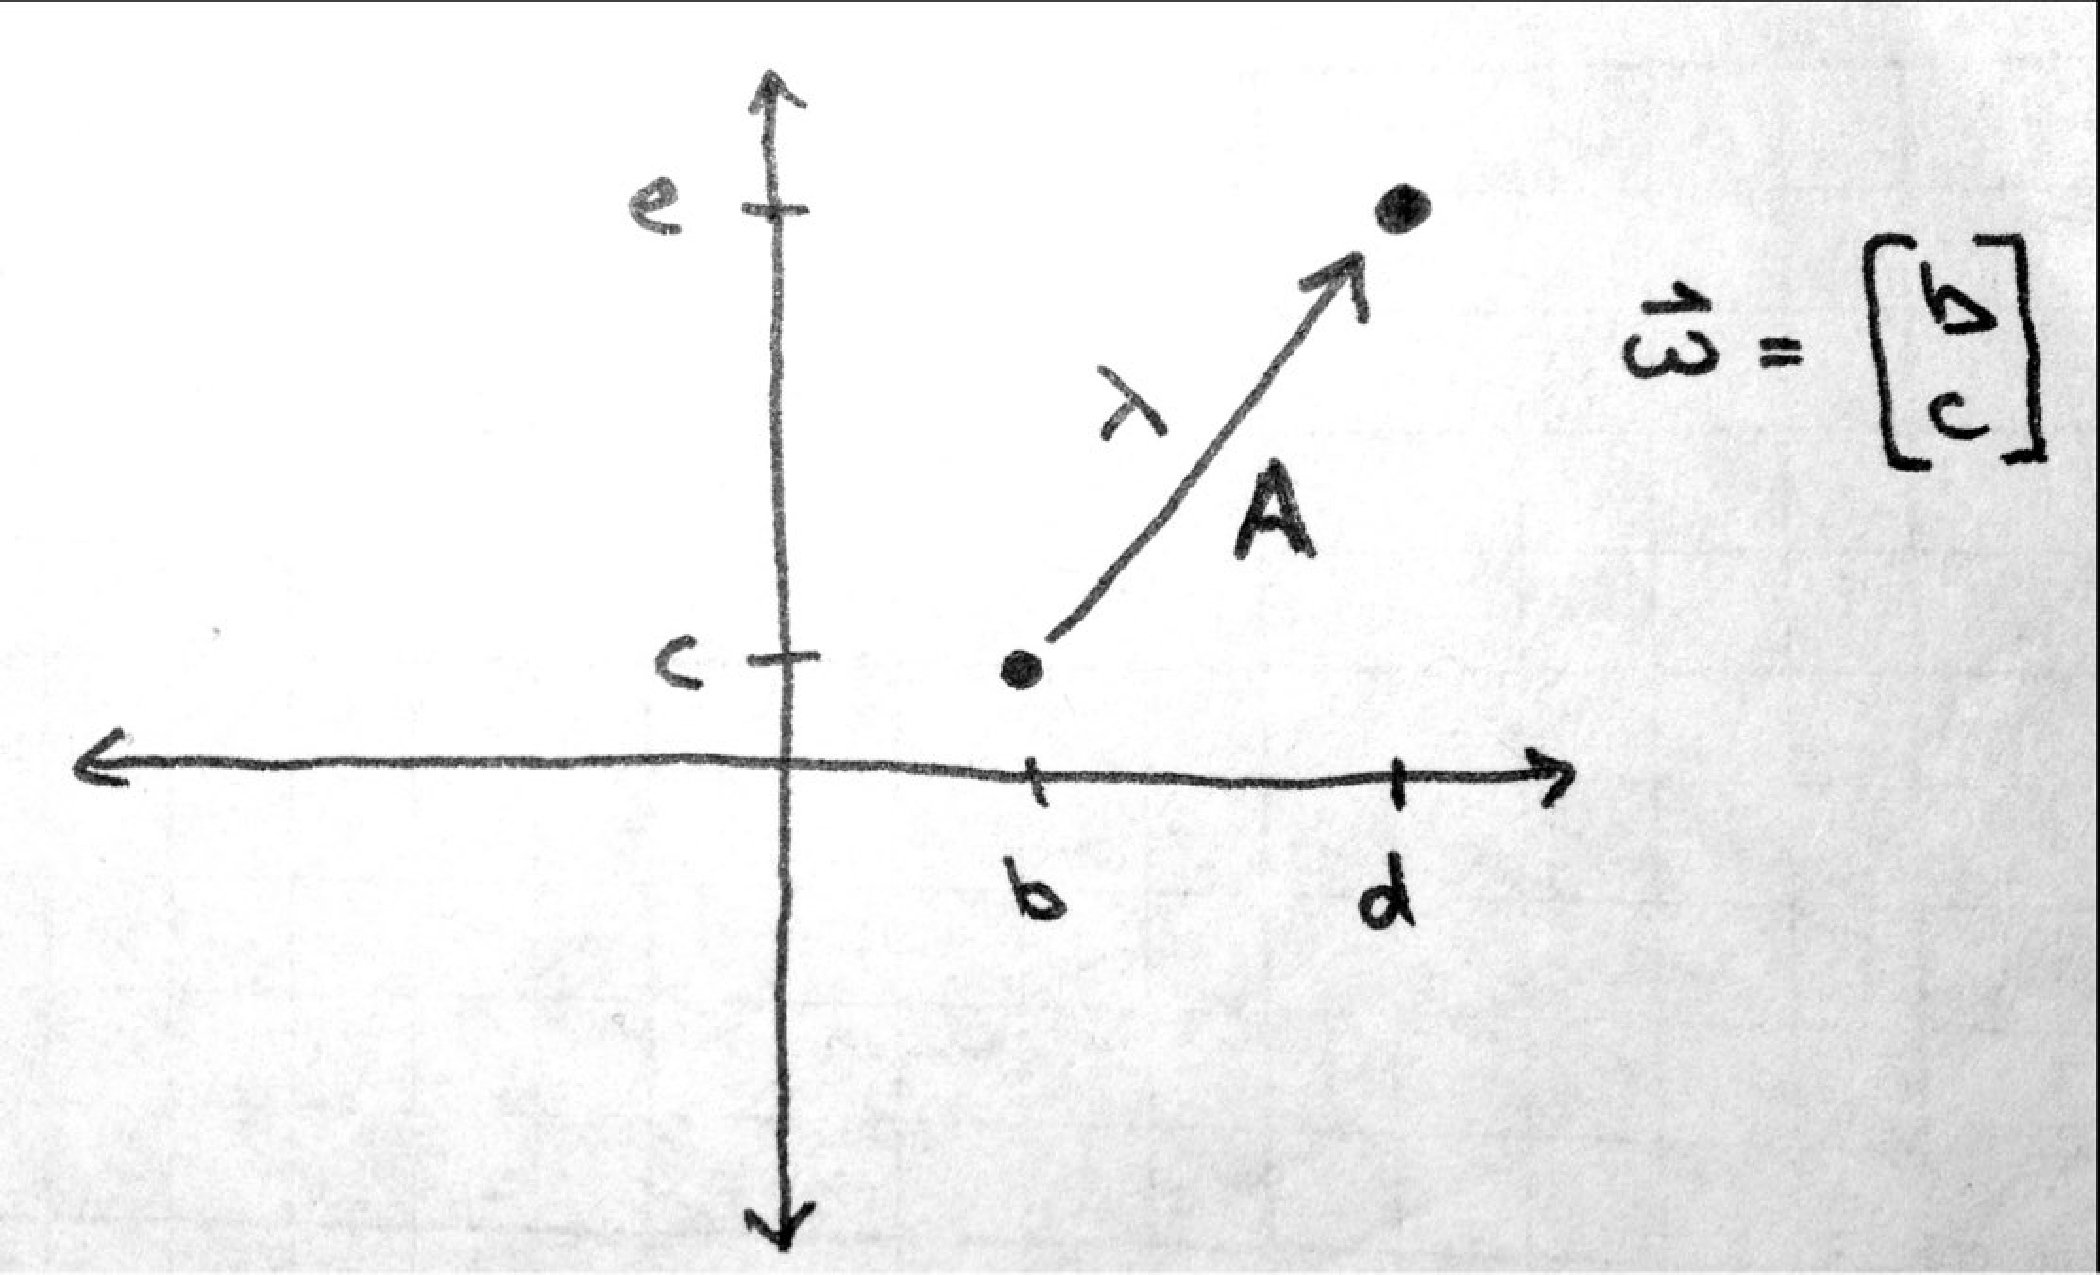
\includegraphics[width=6cm]{figs/eigen1.pdf}
\end{center}

\textbf{Numerical example:}\\
\ind Start at $\vec{w}=\begin{bmatrix} x \\ y \end{bmatrix}=\begin{bmatrix}2 \\ 1 \end{bmatrix} $ and $\mathbf{A} = \begin{bmatrix} 2 & 1 \\ 1 & 3 \end{bmatrix} \qquad  \Rightarrow   \qquad\begin{bmatrix} 2 & 1 \\ 1 & 3 \end{bmatrix} \cdot \begin{bmatrix}2 \\ 1 \end{bmatrix}  = \begin{bmatrix} 4+1 \\ 2+3 \end{bmatrix} =\begin{bmatrix}5 \\ 5 \end{bmatrix}$ 
\begin{center}
	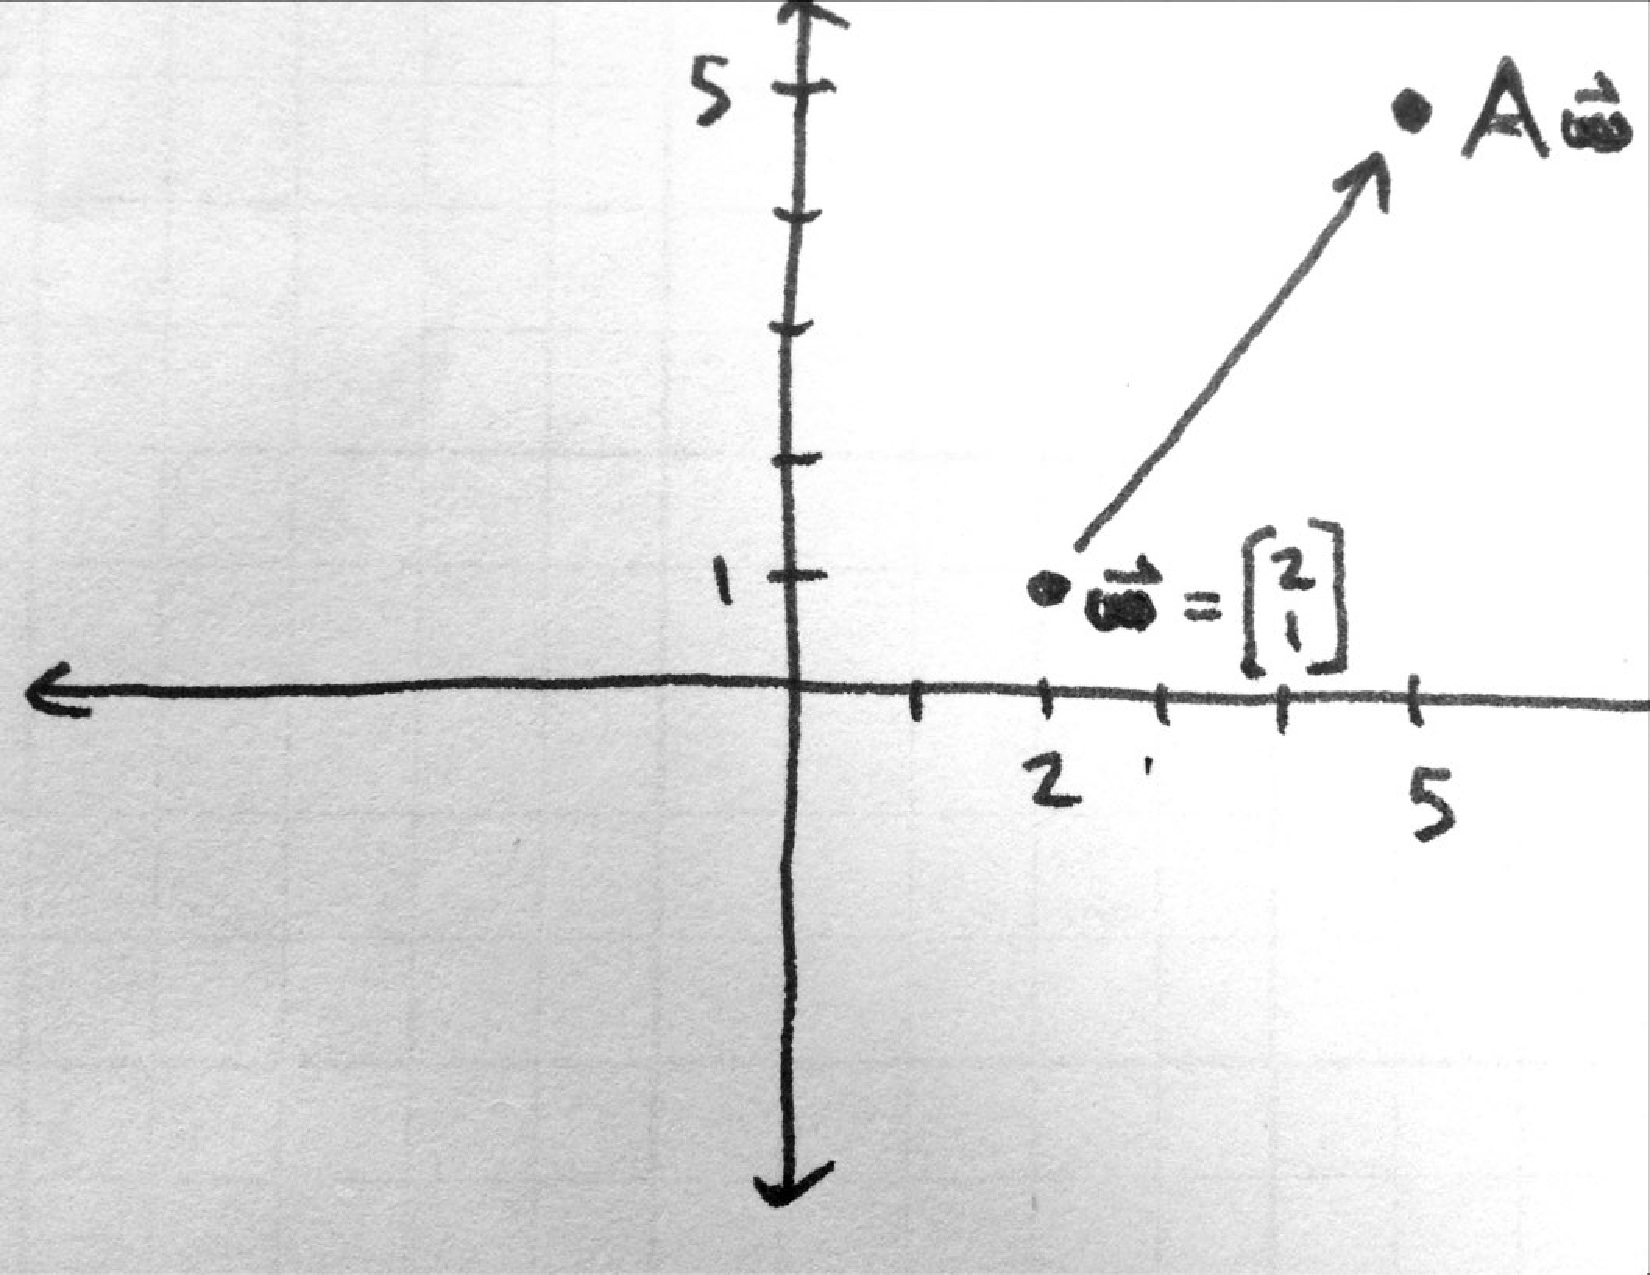
\includegraphics[width=6cm]{figs/eigen2.pdf}
\end{center}
We can do the same thing with $\lambda$ by defining a new coordinate system:
\begin{center}
	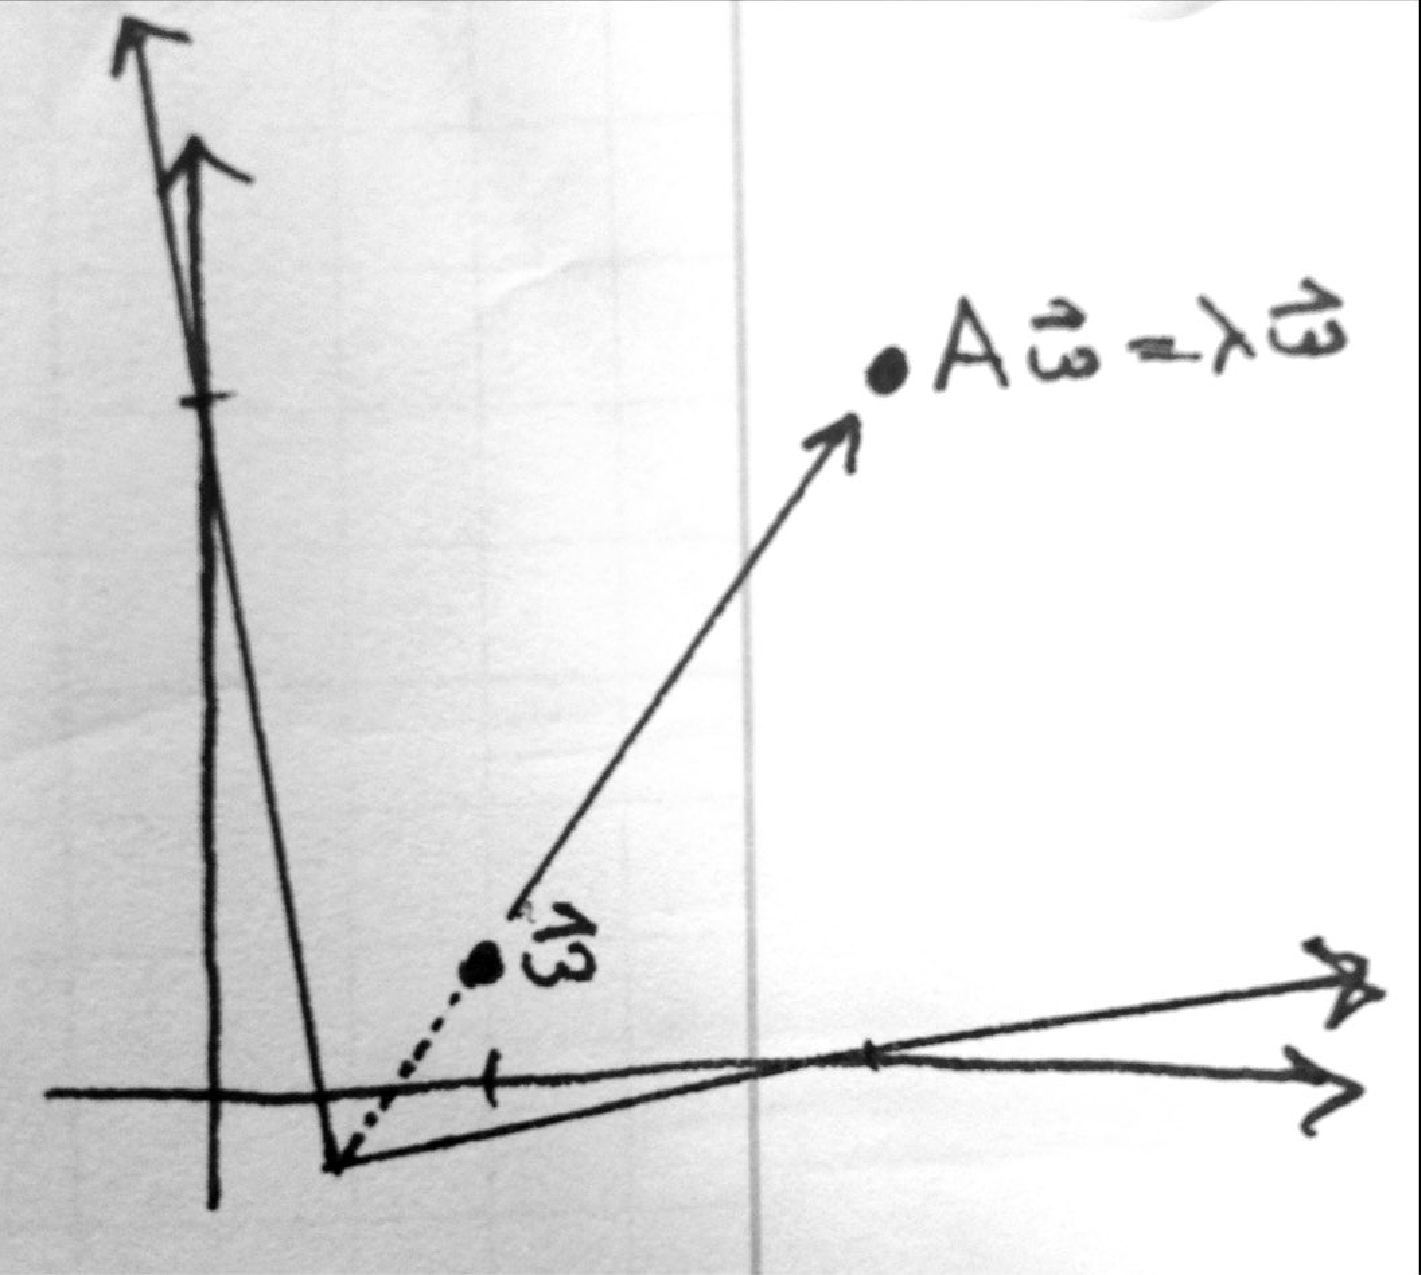
\includegraphics[width=5cm]{figs/eigen3.pdf}
\end{center}

\rule[0.5ex]{\linewidth}{1pt}
\pagebreak

\textbf{How do we determine what $\lambda$ is?}\\
Need to solve:
\begin{equation*}
	\mathbf{A} \vec{w} = \lambda \vec{w} \qquad \Rightarrow \qquad	\mathbf{A} \vec{w} - \lambda \vec{w} = 0
\end{equation*}

First we have to write $\lambda$ in matrix form using \textbf{Identity matrix}:
\begin{equation*}
	\lambda  \mathbf{I} = \lambda \cdot \begin{bmatrix} 1 & 0\\ 0 & 1 	\end{bmatrix} = \begin{bmatrix} \lambda & 0\\ 0 & \lambda 	\end{bmatrix} 
\end{equation*}
Thus:
\begin{align*}
	\mathbf{A} \vec{w} - \lambda \vec{w} = 0\\
	(\mathbf{A} - \lambda \mathbf{I}) \vec{w} = 0
\end{align*}
Thus the solution is either
\begin{equation*}
	\vec{w}=0 \quad \quad \quad \text{or} \quad \quad \quad (\mathbf{A} - \lambda \mathbf{I}) = 0
\end{equation*}

Not interested in $\vec{w} = 0$, but solving $(\mathbf{A} - \lambda \mathbf{I})=0$ isn't any easier than what we started with!\\
However,
\begin{equation*}
	det(\mathbf{A}-\lambda \mathbf{I})=0
\end{equation*}
\ind gives us a way to solve it.

\rule[0.5ex]{\linewidth}{1pt}

\textbf{What is a matrix determinant?}
\begin{equation*}
	det\left( \begin{bmatrix} a & b \\ c & d \end{bmatrix} \right) = a d - b c
\end{equation*}

\begin{equation*}
	det\left( \begin{bmatrix} a & b & c \\ d & e & f \\ g & h & i \end{bmatrix} \right) = aei + bfg + cdh - ceg - fha - ibd
\end{equation*}

Graphical interpretation of the determinant is as a \emph{volume} (or \emph{area} for 2x2 matrices):
\begin{center}
	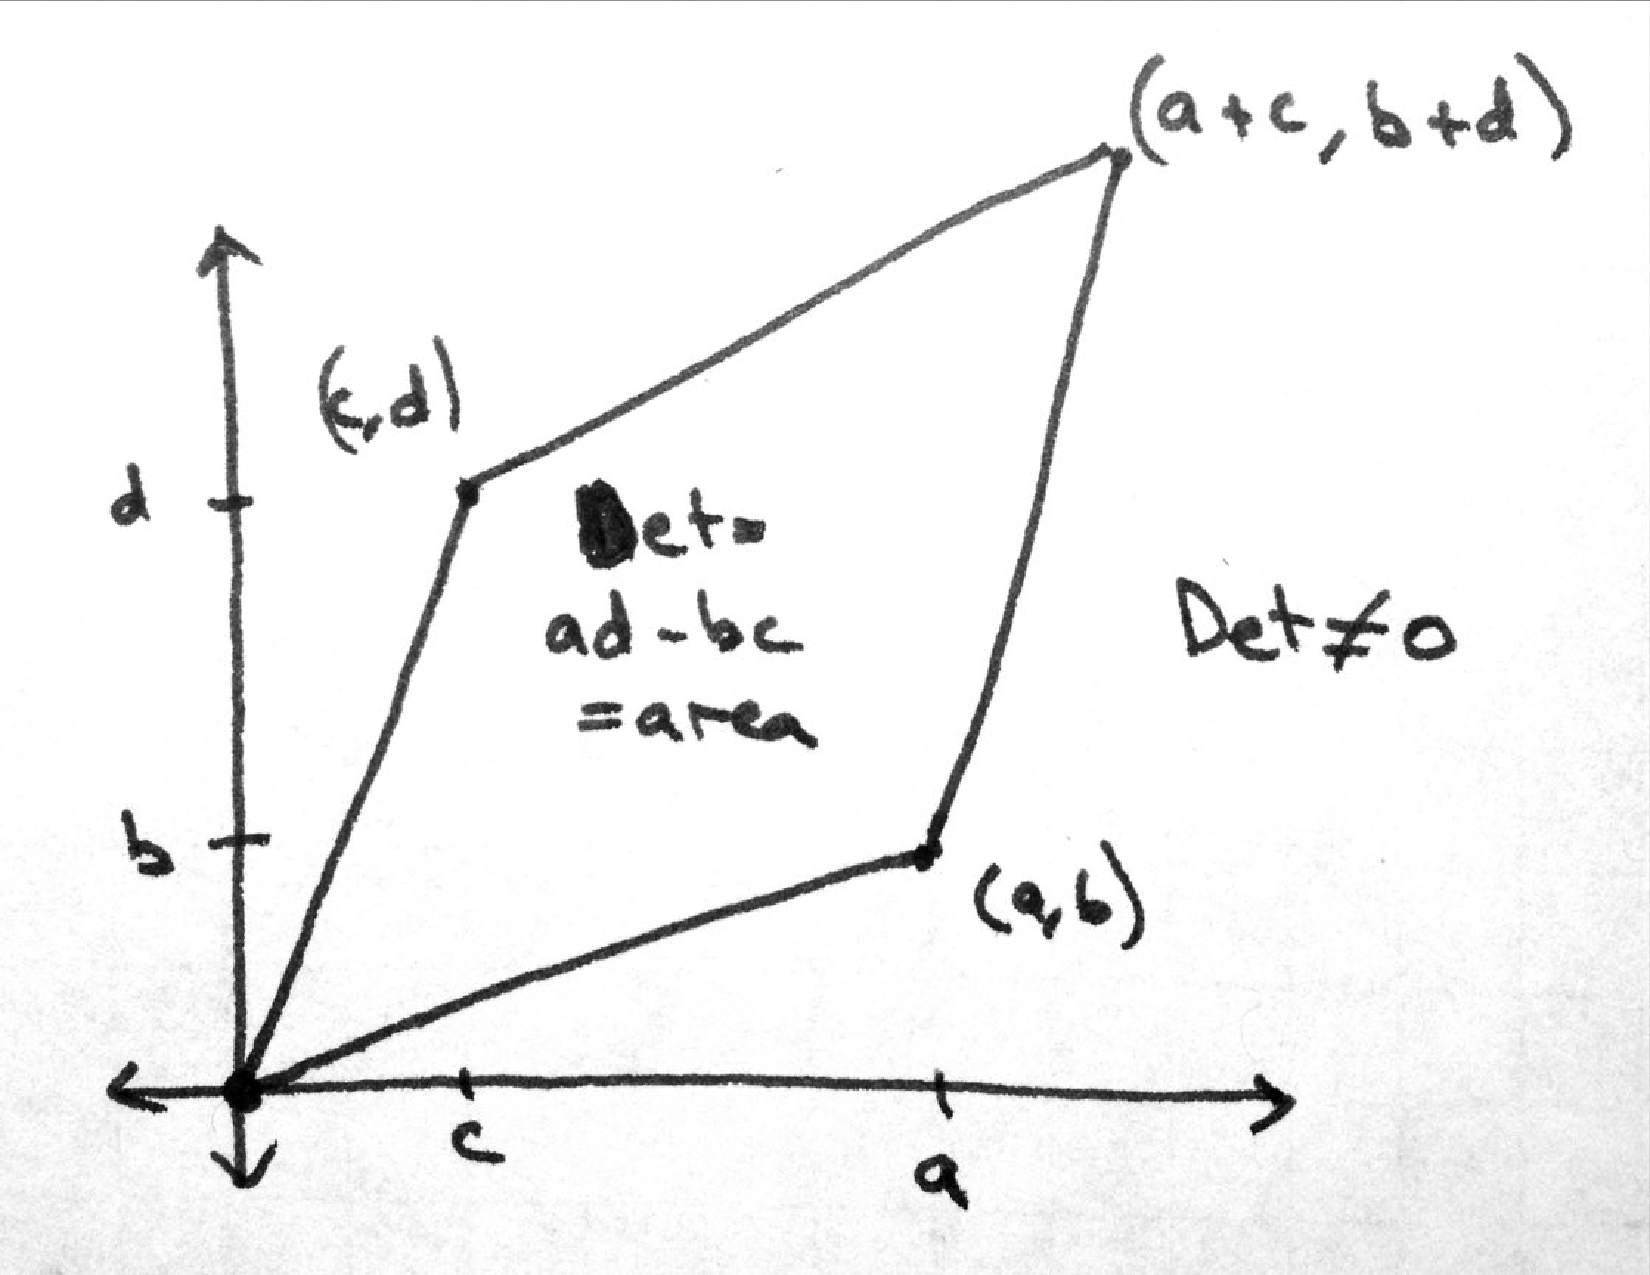
\includegraphics[width=6cm]{figs/DetV.pdf}
		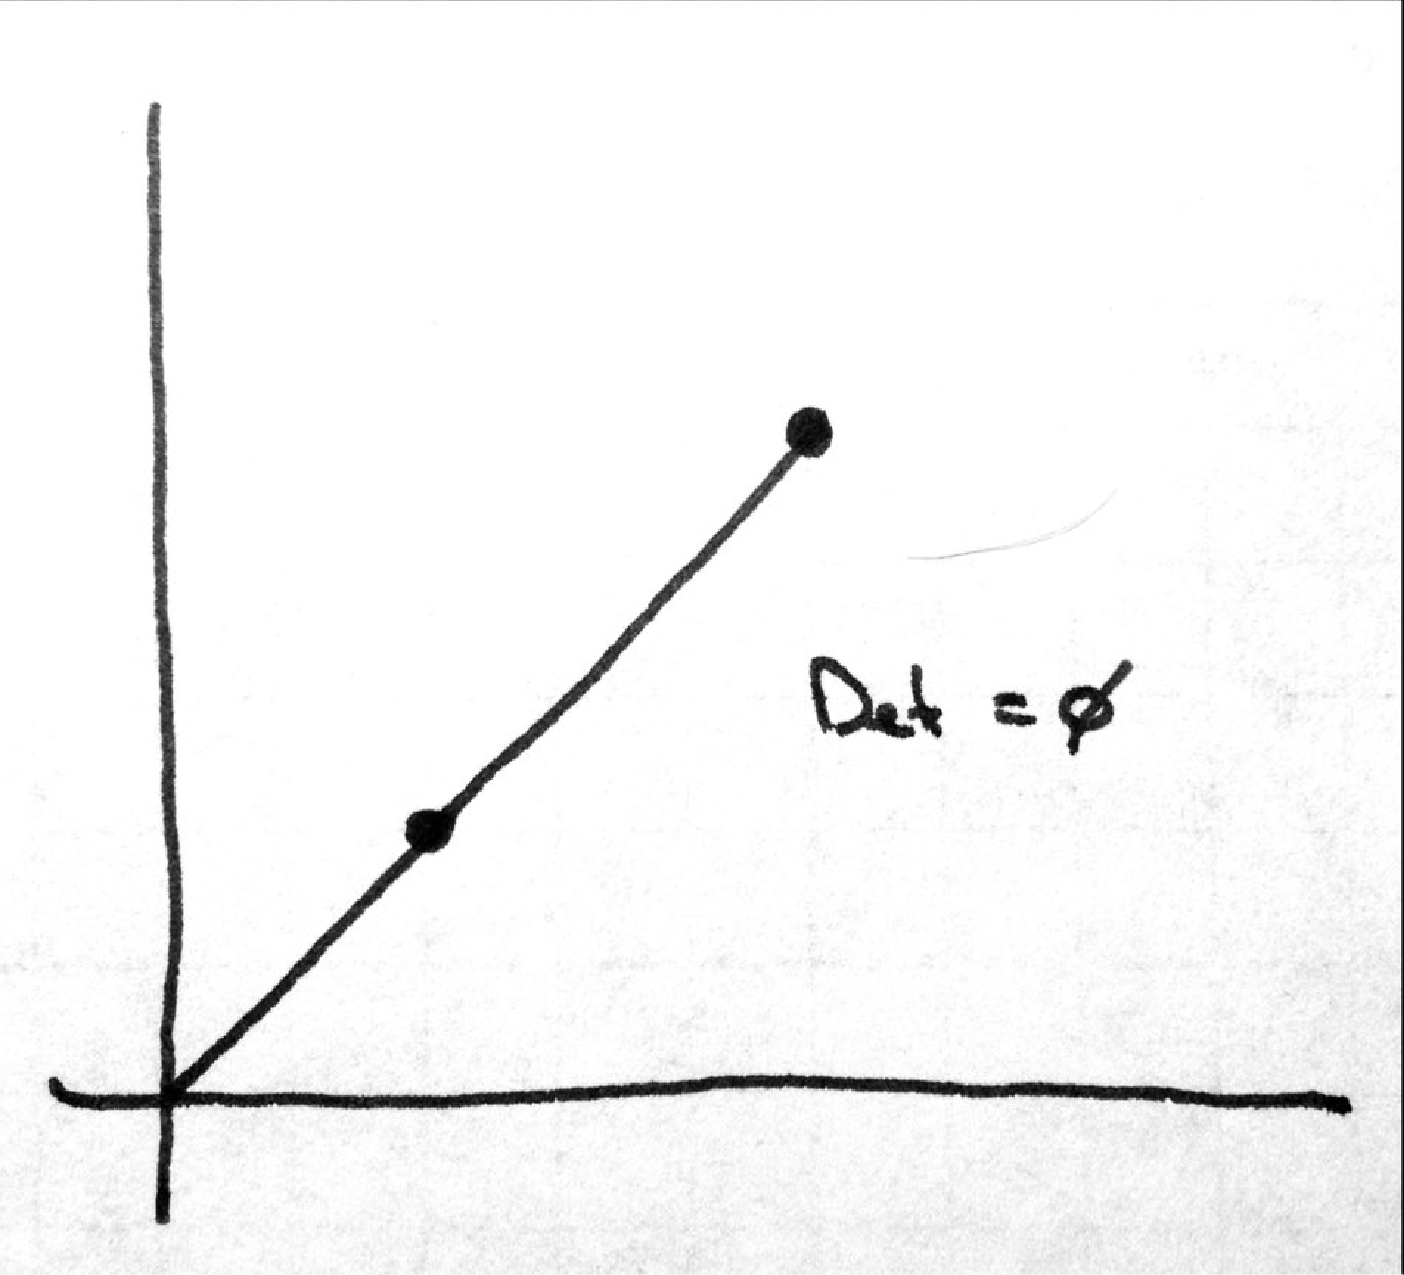
\includegraphics[width=5cm]{figs/Det0.pdf}
\end{center}
\begin{equation*}
	det\left( \begin{bmatrix} 2 & 1 \\ 1 & 3 \end{bmatrix} \right) = 2 \cdot 3 - 1 \cdot 1 = 5 \qquad \qquad \qquad   det\left( \begin{bmatrix} 2 & 1 \\ 4 & 2 \end{bmatrix} \right) = 2 \cdot 2 - 4 \cdot 1 = 0
\end{equation*}

\rule[0.5ex]{\linewidth}{1pt}

\textbf{Back to solving for eigenvalues}\\
If $\lambda$ is just a scaling factor, then the volume of $\mathbf{A}-\lambda \mathbf{I}$ must equal 0.

\begin{align*}
	0&=det(\mathbf{A}-\lambda \mathbf{I})\\
	& = det \left( \begin{bmatrix} A_{11}-\lambda  & A_{12} \\ A_{21} & A_{22} - \lambda \end{bmatrix}\right)\\
	& = (A_{11}-\lambda)(A_{22}-\lambda)- A_{12}A_{12}  \\
	& = \underbrace{\lambda^2 - (A_{11}+A_{22})\lambda + A_{11}A_{22} - A_{12} A_{21}}_{\text{Characteristic equation}}
\end{align*}

\ind $\Rightarrow$ Solve for $\lambda$ by solving the \textbf{characteristic equation}.\\

Solve for $\lambda$ using quadratic formula:
\begin{equation*}
	a x^2 + bx + c = 0 \qquad  \Rightarrow  \qquad x = \frac{-b\pm \sqrt{b^2 - 4ac}}{2a}
\end{equation*}

By defining... \ind (\emph{yes, this is confusing, but it's how it's done in the literature})\\
\begin{equation*}
	\lambda^2 - \underbrace{(A_{11}+A_{22})}_{\text{A}_1}\lambda + \underbrace{A_{11}A_{22} - A_{12} A_{21}}_{\text{A}_2}
\end{equation*}
That is:\ind $\text{A}_1 = A_{11}+A_{22}$ and $\text{A}_2 = A_{11} A_{22} - A_{12} A_{21}$\\

...we have $a=1$, $b=-\text{A}_1$ and $c=\text{A}_2$.
\begin{equation*}
	1 \cdot \lambda^2 + (-\text{A}_1)\lambda + \text{A}_2 = 0 \qquad  \Rightarrow  \qquad  
	 \begin{cases} 
	\lambda_1 = \frac{\text{A}_1 + \sqrt{(-\text{A}_1)^2 - 4\text{A}_2}}{2} \\
	\lambda_2 = \frac{\text{A}_1 - \sqrt{(-\text{A}_1)^2 - 4\text{A}_2}}{2}
	\end{cases}
\end{equation*}

The two solutions to $\lambda$ are called a \textbf{complex conjugate pair}, or  \textbf{complex conjugate roots} (=soltns.).

\rule[0.5ex]{\linewidth}{1pt}
 
\textbf{Compare to single-sp. model}\\
For 1-sp. model we used the sign of the slope $\frac{d \; f(N)}{dN}$ to infer stability:
\begin{equation*}
	\frac{d \; f(N)}{dN} < 0 \quad \Rightarrow \quad \text{stable}
\end{equation*}

Now we're saying that it's the eigenvalues of $\mathbf{A}$ that matter, not the slopes themselves.\\
But remember that the eigenvalues reflect the partial derivative slopes $\frac{\partial \; f_i(\vec{N})}{\partial N_j}$. \\
\ind They reflect the same transformation of the perturbation.\\

In fact, for a 1-sp. model they are exactly the same:\\
\begin{equation*}
	\mathbf{A} \vec{w} = \lambda \vec{w} \qquad \Leftrightarrow \qquad \frac{d \; f(N)}{d N} \cdot  w  = \lambda \cdot w \qquad \Rightarrow \qquad \frac{d \; f(N)}{d N} = \lambda
\end{equation*}

\rule[0.5ex]{\linewidth}{1pt}

\textbf{How do Complex numbers arise?}\\
\begin{equation*}
	\lambda = \frac{\text{A}_1 \pm \sqrt{(-\text{A}_1)^2 - 4\text{A}_2}}{2}
\end{equation*}
When $(-\text{A}_1)^2 < 4 \text{A}_2  \quad \Rightarrow \quad \tfrac{1}{2}(\text{A}_1\pm \sqrt{\text{negative}})$\\
But how do we take the $\sqrt{\phantom{x}}$ of a negative number?\\
\ind $\Rightarrow$ Imaginary unit $i$.
\begin{equation*}
	\boxed{\text{Define }i^2 = -1}
\end{equation*}
\begin{align*}
	\sqrt{-\#} \quad = \quad \sqrt{-1 \cdot \#} \quad = \quad \sqrt{i^2\#} \quad = \quad \sqrt{i^2} \sqrt{\#} = \quad i \sqrt{\#}\\
	\text{e.g.,} \quad	\sqrt{-4} \quad = \quad \sqrt{-1 \cdot 4} \quad = \quad \sqrt{i^2 4} \quad = \quad i \sqrt{4} \quad = \quad i2
\end{align*}
\begin{equation*}
	\lambda = \tfrac{1}{2}\text{A}_1 \pm \tfrac{1}{2}\sqrt{(-\text{A}_1)^2 - 4\text{A}_2} \; i
\end{equation*}

There is nothing `imaginary' about imaginary numbers!  They're as `real' as negative numbers!\\
\ind \emph{Real} numbers are just counts or fractional counts \\
\ind \ind (= easy to think about as an amount of something).\\
\ind \ind Can you imagine how much an amount of -10 is?  No!\\
\ind \ind Negative counts don't exist.  They're a mathematical convenience to subtract amounts.
\ind \emph{Imaginary} numbers exist as much as negative numbers do! \\
\ind \ind They're a mathematical convenience to allow taking roots of negative numbers.\\

\emph{In order to solve... we invented...}
\begin{align*}
	&\begin{rcases}
	x-5 = 0 \qquad &\Rightarrow \qquad \text{Integers}\\
	x+5 = 0 \qquad &\Rightarrow \qquad \text{Negative integers}\\
	\end{rcases}
	\quad\text{(Real numbers)}\\
	&2x = 1 \qquad \Rightarrow \qquad \text{Rational numbers (fractions, quotients of integers)}\\
	&x^2 = 2 \qquad \Rightarrow \qquad \text{Irrational numbers (can't be expressed as fractions, e.g., }\sqrt{2}, \pi, e)\\
	&x^2= -1 \qquad \Rightarrow \qquad \text{Imaginary numbers.}
\end{align*}
Think about imaginary numbers as representing a different number dimension:
 \begin{center}
 	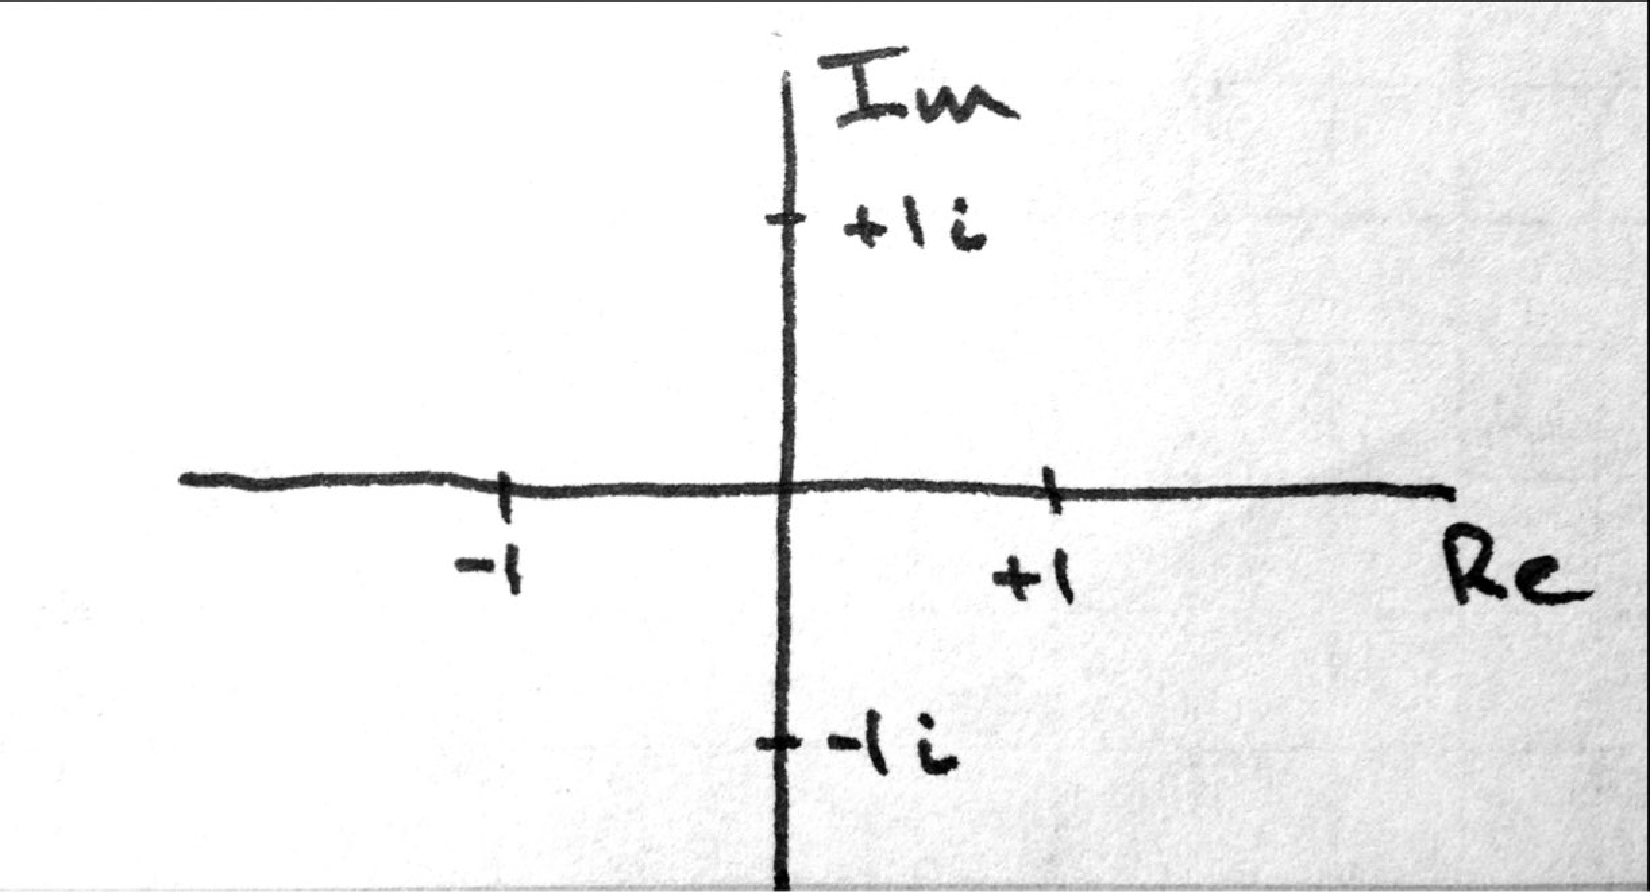
\includegraphics[width=5cm]{figs/Imag.pdf}
 \end{center}
 
\rule[0.5ex]{\linewidth}{1pt}

\textbf{Why do imaginary parts indicate oscillations?}\\
Remember that $\lambda$ represents dynamics of the perturbation:
\begin{equation*}
	\vec{n}_t = \vec{n}_0 e^{\lambda t}
\end{equation*}
With a complex part:
\begin{equation*}
	\vec{n}_t = \vec{n}_0 e^{(a \pm bi) t} = e^{at} \cdot e^{i bt}
\end{equation*}

From the theory of complex numbers:
\begin{align*}
	e^{i \Theta} &= \cos \Theta + i \sin \Theta
\end{align*}
Thinking  of $bt$ as $\Theta$ gives:
\begin{equation*}
	e^{i bt} = \cos (bt) + i\sin (bt)
\end{equation*} 
Thus:
\begin{equation*}
	e^{(a \pm bi) t} =  e^{at} \cdot  [\cos (bt) \pm i\sin (bt)]
\end{equation*} 

Therefore, $a$ controls stability
\begin{align*}
	a<0 &\Rightarrow \quad \text{oscillations will dampen}\\
	a>0 &\Rightarrow \quad \text{oscillations will amplify}\\
	a=0 &\Rightarrow \quad \text{neutral stability with cycles}
\end{align*}
And $b$ controls the \emph{frequency} of the oscillations.

 \rule[0.5ex]{\linewidth}{1pt}
\textbf{n-spp. stability}\\
 Note that we can determine the eigenvalues of an arbitrary-sized square matrix (not just 2-by-2).\\
 We can therefore use eigenvalues to evaluate the local stability of any system of equations for any number of interacting species!
 
\rule[0.5ex]{\linewidth}{1pt}
\rule[0.5ex]{\linewidth}{1pt}

\end{document}